\documentclass[11pt]{article}

    \usepackage[breakable]{tcolorbox}
    \usepackage{parskip} % Stop auto-indenting (to mimic markdown behaviour)
    
    \usepackage{iftex}
    \ifPDFTeX
    	\usepackage[T1]{fontenc}
    	\usepackage{mathpazo}
    \else
    	\usepackage{fontspec}
    \fi

    % Basic figure setup, for now with no caption control since it's done
    % automatically by Pandoc (which extracts ![](path) syntax from Markdown).
    \usepackage{graphicx}
    % Maintain compatibility with old templates. Remove in nbconvert 6.0
    \let\Oldincludegraphics\includegraphics
    % Ensure that by default, figures have no caption (until we provide a
    % proper Figure object with a Caption API and a way to capture that
    % in the conversion process - todo).
    \usepackage{caption}
    \DeclareCaptionFormat{nocaption}{}
    \captionsetup{format=nocaption,aboveskip=0pt,belowskip=0pt}

    \usepackage{float}
    \floatplacement{figure}{H} % forces figures to be placed at the correct location
    \usepackage{xcolor} % Allow colors to be defined
    \usepackage{enumerate} % Needed for markdown enumerations to work
    \usepackage{geometry} % Used to adjust the document margins
    \usepackage{amsmath} % Equations
    \usepackage{amssymb} % Equations
    \usepackage{textcomp} % defines textquotesingle
    % Hack from http://tex.stackexchange.com/a/47451/13684:
    \AtBeginDocument{%
        \def\PYZsq{\textquotesingle}% Upright quotes in Pygmentized code
    }
    \usepackage{upquote} % Upright quotes for verbatim code
    \usepackage{eurosym} % defines \euro
    \usepackage[mathletters]{ucs} % Extended unicode (utf-8) support
    \usepackage{fancyvrb} % verbatim replacement that allows latex
    \usepackage{grffile} % extends the file name processing of package graphics 
                         % to support a larger range
    \makeatletter % fix for old versions of grffile with XeLaTeX
    \@ifpackagelater{grffile}{2019/11/01}
    {
      % Do nothing on new versions
    }
    {
      \def\Gread@@xetex#1{%
        \IfFileExists{"\Gin@base".bb}%
        {\Gread@eps{\Gin@base.bb}}%
        {\Gread@@xetex@aux#1}%
      }
    }
    \makeatother
    \usepackage[Export]{adjustbox} % Used to constrain images to a maximum size
    \adjustboxset{max size={0.9\linewidth}{0.9\paperheight}}

    % The hyperref package gives us a pdf with properly built
    % internal navigation ('pdf bookmarks' for the table of contents,
    % internal cross-reference links, web links for URLs, etc.)
    \usepackage{hyperref}
    % The default LaTeX title has an obnoxious amount of whitespace. By default,
    % titling removes some of it. It also provides customization options.
    \usepackage{titling}
    \usepackage{longtable} % longtable support required by pandoc >1.10
    \usepackage{booktabs}  % table support for pandoc > 1.12.2
    \usepackage[inline]{enumitem} % IRkernel/repr support (it uses the enumerate* environment)
    \usepackage[normalem]{ulem} % ulem is needed to support strikethroughs (\sout)
                                % normalem makes italics be italics, not underlines
    \usepackage{mathrsfs}
    

    
    % Colors for the hyperref package
    \definecolor{urlcolor}{rgb}{0,.145,.698}
    \definecolor{linkcolor}{rgb}{.71,0.21,0.01}
    \definecolor{citecolor}{rgb}{.12,.54,.11}

    % ANSI colors
    \definecolor{ansi-black}{HTML}{3E424D}
    \definecolor{ansi-black-intense}{HTML}{282C36}
    \definecolor{ansi-red}{HTML}{E75C58}
    \definecolor{ansi-red-intense}{HTML}{B22B31}
    \definecolor{ansi-green}{HTML}{00A250}
    \definecolor{ansi-green-intense}{HTML}{007427}
    \definecolor{ansi-yellow}{HTML}{DDB62B}
    \definecolor{ansi-yellow-intense}{HTML}{B27D12}
    \definecolor{ansi-blue}{HTML}{208FFB}
    \definecolor{ansi-blue-intense}{HTML}{0065CA}
    \definecolor{ansi-magenta}{HTML}{D160C4}
    \definecolor{ansi-magenta-intense}{HTML}{A03196}
    \definecolor{ansi-cyan}{HTML}{60C6C8}
    \definecolor{ansi-cyan-intense}{HTML}{258F8F}
    \definecolor{ansi-white}{HTML}{C5C1B4}
    \definecolor{ansi-white-intense}{HTML}{A1A6B2}
    \definecolor{ansi-default-inverse-fg}{HTML}{FFFFFF}
    \definecolor{ansi-default-inverse-bg}{HTML}{000000}

    % common color for the border for error outputs.
    \definecolor{outerrorbackground}{HTML}{FFDFDF}

    % commands and environments needed by pandoc snippets
    % extracted from the output of `pandoc -s`
    \providecommand{\tightlist}{%
      \setlength{\itemsep}{0pt}\setlength{\parskip}{0pt}}
    \DefineVerbatimEnvironment{Highlighting}{Verbatim}{commandchars=\\\{\}}
    % Add ',fontsize=\small' for more characters per line
    \newenvironment{Shaded}{}{}
    \newcommand{\KeywordTok}[1]{\textcolor[rgb]{0.00,0.44,0.13}{\textbf{{#1}}}}
    \newcommand{\DataTypeTok}[1]{\textcolor[rgb]{0.56,0.13,0.00}{{#1}}}
    \newcommand{\DecValTok}[1]{\textcolor[rgb]{0.25,0.63,0.44}{{#1}}}
    \newcommand{\BaseNTok}[1]{\textcolor[rgb]{0.25,0.63,0.44}{{#1}}}
    \newcommand{\FloatTok}[1]{\textcolor[rgb]{0.25,0.63,0.44}{{#1}}}
    \newcommand{\CharTok}[1]{\textcolor[rgb]{0.25,0.44,0.63}{{#1}}}
    \newcommand{\StringTok}[1]{\textcolor[rgb]{0.25,0.44,0.63}{{#1}}}
    \newcommand{\CommentTok}[1]{\textcolor[rgb]{0.38,0.63,0.69}{\textit{{#1}}}}
    \newcommand{\OtherTok}[1]{\textcolor[rgb]{0.00,0.44,0.13}{{#1}}}
    \newcommand{\AlertTok}[1]{\textcolor[rgb]{1.00,0.00,0.00}{\textbf{{#1}}}}
    \newcommand{\FunctionTok}[1]{\textcolor[rgb]{0.02,0.16,0.49}{{#1}}}
    \newcommand{\RegionMarkerTok}[1]{{#1}}
    \newcommand{\ErrorTok}[1]{\textcolor[rgb]{1.00,0.00,0.00}{\textbf{{#1}}}}
    \newcommand{\NormalTok}[1]{{#1}}
    
    % Additional commands for more recent versions of Pandoc
    \newcommand{\ConstantTok}[1]{\textcolor[rgb]{0.53,0.00,0.00}{{#1}}}
    \newcommand{\SpecialCharTok}[1]{\textcolor[rgb]{0.25,0.44,0.63}{{#1}}}
    \newcommand{\VerbatimStringTok}[1]{\textcolor[rgb]{0.25,0.44,0.63}{{#1}}}
    \newcommand{\SpecialStringTok}[1]{\textcolor[rgb]{0.73,0.40,0.53}{{#1}}}
    \newcommand{\ImportTok}[1]{{#1}}
    \newcommand{\DocumentationTok}[1]{\textcolor[rgb]{0.73,0.13,0.13}{\textit{{#1}}}}
    \newcommand{\AnnotationTok}[1]{\textcolor[rgb]{0.38,0.63,0.69}{\textbf{\textit{{#1}}}}}
    \newcommand{\CommentVarTok}[1]{\textcolor[rgb]{0.38,0.63,0.69}{\textbf{\textit{{#1}}}}}
    \newcommand{\VariableTok}[1]{\textcolor[rgb]{0.10,0.09,0.49}{{#1}}}
    \newcommand{\ControlFlowTok}[1]{\textcolor[rgb]{0.00,0.44,0.13}{\textbf{{#1}}}}
    \newcommand{\OperatorTok}[1]{\textcolor[rgb]{0.40,0.40,0.40}{{#1}}}
    \newcommand{\BuiltInTok}[1]{{#1}}
    \newcommand{\ExtensionTok}[1]{{#1}}
    \newcommand{\PreprocessorTok}[1]{\textcolor[rgb]{0.74,0.48,0.00}{{#1}}}
    \newcommand{\AttributeTok}[1]{\textcolor[rgb]{0.49,0.56,0.16}{{#1}}}
    \newcommand{\InformationTok}[1]{\textcolor[rgb]{0.38,0.63,0.69}{\textbf{\textit{{#1}}}}}
    \newcommand{\WarningTok}[1]{\textcolor[rgb]{0.38,0.63,0.69}{\textbf{\textit{{#1}}}}}
    
    
    % Define a nice break command that doesn't care if a line doesn't already
    % exist.
    \def\br{\hspace*{\fill} \\* }
    % Math Jax compatibility definitions
    \def\gt{>}
    \def\lt{<}
    \let\Oldtex\TeX
    \let\Oldlatex\LaTeX
    \renewcommand{\TeX}{\textrm{\Oldtex}}
    \renewcommand{\LaTeX}{\textrm{\Oldlatex}}
    % Document parameters
    % Document title
    \title{Sir Tet Tetris AI Playground and Deep Q Learning agents for Tetris}
    
    
    
    
    
% Pygments definitions
\makeatletter
\def\PY@reset{\let\PY@it=\relax \let\PY@bf=\relax%
    \let\PY@ul=\relax \let\PY@tc=\relax%
    \let\PY@bc=\relax \let\PY@ff=\relax}
\def\PY@tok#1{\csname PY@tok@#1\endcsname}
\def\PY@toks#1+{\ifx\relax#1\empty\else%
    \PY@tok{#1}\expandafter\PY@toks\fi}
\def\PY@do#1{\PY@bc{\PY@tc{\PY@ul{%
    \PY@it{\PY@bf{\PY@ff{#1}}}}}}}
\def\PY#1#2{\PY@reset\PY@toks#1+\relax+\PY@do{#2}}

\expandafter\def\csname PY@tok@w\endcsname{\def\PY@tc##1{\textcolor[rgb]{0.73,0.73,0.73}{##1}}}
\expandafter\def\csname PY@tok@c\endcsname{\let\PY@it=\textit\def\PY@tc##1{\textcolor[rgb]{0.25,0.50,0.50}{##1}}}
\expandafter\def\csname PY@tok@cp\endcsname{\def\PY@tc##1{\textcolor[rgb]{0.74,0.48,0.00}{##1}}}
\expandafter\def\csname PY@tok@k\endcsname{\let\PY@bf=\textbf\def\PY@tc##1{\textcolor[rgb]{0.00,0.50,0.00}{##1}}}
\expandafter\def\csname PY@tok@kp\endcsname{\def\PY@tc##1{\textcolor[rgb]{0.00,0.50,0.00}{##1}}}
\expandafter\def\csname PY@tok@kt\endcsname{\def\PY@tc##1{\textcolor[rgb]{0.69,0.00,0.25}{##1}}}
\expandafter\def\csname PY@tok@o\endcsname{\def\PY@tc##1{\textcolor[rgb]{0.40,0.40,0.40}{##1}}}
\expandafter\def\csname PY@tok@ow\endcsname{\let\PY@bf=\textbf\def\PY@tc##1{\textcolor[rgb]{0.67,0.13,1.00}{##1}}}
\expandafter\def\csname PY@tok@nb\endcsname{\def\PY@tc##1{\textcolor[rgb]{0.00,0.50,0.00}{##1}}}
\expandafter\def\csname PY@tok@nf\endcsname{\def\PY@tc##1{\textcolor[rgb]{0.00,0.00,1.00}{##1}}}
\expandafter\def\csname PY@tok@nc\endcsname{\let\PY@bf=\textbf\def\PY@tc##1{\textcolor[rgb]{0.00,0.00,1.00}{##1}}}
\expandafter\def\csname PY@tok@nn\endcsname{\let\PY@bf=\textbf\def\PY@tc##1{\textcolor[rgb]{0.00,0.00,1.00}{##1}}}
\expandafter\def\csname PY@tok@ne\endcsname{\let\PY@bf=\textbf\def\PY@tc##1{\textcolor[rgb]{0.82,0.25,0.23}{##1}}}
\expandafter\def\csname PY@tok@nv\endcsname{\def\PY@tc##1{\textcolor[rgb]{0.10,0.09,0.49}{##1}}}
\expandafter\def\csname PY@tok@no\endcsname{\def\PY@tc##1{\textcolor[rgb]{0.53,0.00,0.00}{##1}}}
\expandafter\def\csname PY@tok@nl\endcsname{\def\PY@tc##1{\textcolor[rgb]{0.63,0.63,0.00}{##1}}}
\expandafter\def\csname PY@tok@ni\endcsname{\let\PY@bf=\textbf\def\PY@tc##1{\textcolor[rgb]{0.60,0.60,0.60}{##1}}}
\expandafter\def\csname PY@tok@na\endcsname{\def\PY@tc##1{\textcolor[rgb]{0.49,0.56,0.16}{##1}}}
\expandafter\def\csname PY@tok@nt\endcsname{\let\PY@bf=\textbf\def\PY@tc##1{\textcolor[rgb]{0.00,0.50,0.00}{##1}}}
\expandafter\def\csname PY@tok@nd\endcsname{\def\PY@tc##1{\textcolor[rgb]{0.67,0.13,1.00}{##1}}}
\expandafter\def\csname PY@tok@s\endcsname{\def\PY@tc##1{\textcolor[rgb]{0.73,0.13,0.13}{##1}}}
\expandafter\def\csname PY@tok@sd\endcsname{\let\PY@it=\textit\def\PY@tc##1{\textcolor[rgb]{0.73,0.13,0.13}{##1}}}
\expandafter\def\csname PY@tok@si\endcsname{\let\PY@bf=\textbf\def\PY@tc##1{\textcolor[rgb]{0.73,0.40,0.53}{##1}}}
\expandafter\def\csname PY@tok@se\endcsname{\let\PY@bf=\textbf\def\PY@tc##1{\textcolor[rgb]{0.73,0.40,0.13}{##1}}}
\expandafter\def\csname PY@tok@sr\endcsname{\def\PY@tc##1{\textcolor[rgb]{0.73,0.40,0.53}{##1}}}
\expandafter\def\csname PY@tok@ss\endcsname{\def\PY@tc##1{\textcolor[rgb]{0.10,0.09,0.49}{##1}}}
\expandafter\def\csname PY@tok@sx\endcsname{\def\PY@tc##1{\textcolor[rgb]{0.00,0.50,0.00}{##1}}}
\expandafter\def\csname PY@tok@m\endcsname{\def\PY@tc##1{\textcolor[rgb]{0.40,0.40,0.40}{##1}}}
\expandafter\def\csname PY@tok@gh\endcsname{\let\PY@bf=\textbf\def\PY@tc##1{\textcolor[rgb]{0.00,0.00,0.50}{##1}}}
\expandafter\def\csname PY@tok@gu\endcsname{\let\PY@bf=\textbf\def\PY@tc##1{\textcolor[rgb]{0.50,0.00,0.50}{##1}}}
\expandafter\def\csname PY@tok@gd\endcsname{\def\PY@tc##1{\textcolor[rgb]{0.63,0.00,0.00}{##1}}}
\expandafter\def\csname PY@tok@gi\endcsname{\def\PY@tc##1{\textcolor[rgb]{0.00,0.63,0.00}{##1}}}
\expandafter\def\csname PY@tok@gr\endcsname{\def\PY@tc##1{\textcolor[rgb]{1.00,0.00,0.00}{##1}}}
\expandafter\def\csname PY@tok@ge\endcsname{\let\PY@it=\textit}
\expandafter\def\csname PY@tok@gs\endcsname{\let\PY@bf=\textbf}
\expandafter\def\csname PY@tok@gp\endcsname{\let\PY@bf=\textbf\def\PY@tc##1{\textcolor[rgb]{0.00,0.00,0.50}{##1}}}
\expandafter\def\csname PY@tok@go\endcsname{\def\PY@tc##1{\textcolor[rgb]{0.53,0.53,0.53}{##1}}}
\expandafter\def\csname PY@tok@gt\endcsname{\def\PY@tc##1{\textcolor[rgb]{0.00,0.27,0.87}{##1}}}
\expandafter\def\csname PY@tok@err\endcsname{\def\PY@bc##1{\setlength{\fboxsep}{0pt}\fcolorbox[rgb]{1.00,0.00,0.00}{1,1,1}{\strut ##1}}}
\expandafter\def\csname PY@tok@kc\endcsname{\let\PY@bf=\textbf\def\PY@tc##1{\textcolor[rgb]{0.00,0.50,0.00}{##1}}}
\expandafter\def\csname PY@tok@kd\endcsname{\let\PY@bf=\textbf\def\PY@tc##1{\textcolor[rgb]{0.00,0.50,0.00}{##1}}}
\expandafter\def\csname PY@tok@kn\endcsname{\let\PY@bf=\textbf\def\PY@tc##1{\textcolor[rgb]{0.00,0.50,0.00}{##1}}}
\expandafter\def\csname PY@tok@kr\endcsname{\let\PY@bf=\textbf\def\PY@tc##1{\textcolor[rgb]{0.00,0.50,0.00}{##1}}}
\expandafter\def\csname PY@tok@bp\endcsname{\def\PY@tc##1{\textcolor[rgb]{0.00,0.50,0.00}{##1}}}
\expandafter\def\csname PY@tok@fm\endcsname{\def\PY@tc##1{\textcolor[rgb]{0.00,0.00,1.00}{##1}}}
\expandafter\def\csname PY@tok@vc\endcsname{\def\PY@tc##1{\textcolor[rgb]{0.10,0.09,0.49}{##1}}}
\expandafter\def\csname PY@tok@vg\endcsname{\def\PY@tc##1{\textcolor[rgb]{0.10,0.09,0.49}{##1}}}
\expandafter\def\csname PY@tok@vi\endcsname{\def\PY@tc##1{\textcolor[rgb]{0.10,0.09,0.49}{##1}}}
\expandafter\def\csname PY@tok@vm\endcsname{\def\PY@tc##1{\textcolor[rgb]{0.10,0.09,0.49}{##1}}}
\expandafter\def\csname PY@tok@sa\endcsname{\def\PY@tc##1{\textcolor[rgb]{0.73,0.13,0.13}{##1}}}
\expandafter\def\csname PY@tok@sb\endcsname{\def\PY@tc##1{\textcolor[rgb]{0.73,0.13,0.13}{##1}}}
\expandafter\def\csname PY@tok@sc\endcsname{\def\PY@tc##1{\textcolor[rgb]{0.73,0.13,0.13}{##1}}}
\expandafter\def\csname PY@tok@dl\endcsname{\def\PY@tc##1{\textcolor[rgb]{0.73,0.13,0.13}{##1}}}
\expandafter\def\csname PY@tok@s2\endcsname{\def\PY@tc##1{\textcolor[rgb]{0.73,0.13,0.13}{##1}}}
\expandafter\def\csname PY@tok@sh\endcsname{\def\PY@tc##1{\textcolor[rgb]{0.73,0.13,0.13}{##1}}}
\expandafter\def\csname PY@tok@s1\endcsname{\def\PY@tc##1{\textcolor[rgb]{0.73,0.13,0.13}{##1}}}
\expandafter\def\csname PY@tok@mb\endcsname{\def\PY@tc##1{\textcolor[rgb]{0.40,0.40,0.40}{##1}}}
\expandafter\def\csname PY@tok@mf\endcsname{\def\PY@tc##1{\textcolor[rgb]{0.40,0.40,0.40}{##1}}}
\expandafter\def\csname PY@tok@mh\endcsname{\def\PY@tc##1{\textcolor[rgb]{0.40,0.40,0.40}{##1}}}
\expandafter\def\csname PY@tok@mi\endcsname{\def\PY@tc##1{\textcolor[rgb]{0.40,0.40,0.40}{##1}}}
\expandafter\def\csname PY@tok@il\endcsname{\def\PY@tc##1{\textcolor[rgb]{0.40,0.40,0.40}{##1}}}
\expandafter\def\csname PY@tok@mo\endcsname{\def\PY@tc##1{\textcolor[rgb]{0.40,0.40,0.40}{##1}}}
\expandafter\def\csname PY@tok@ch\endcsname{\let\PY@it=\textit\def\PY@tc##1{\textcolor[rgb]{0.25,0.50,0.50}{##1}}}
\expandafter\def\csname PY@tok@cm\endcsname{\let\PY@it=\textit\def\PY@tc##1{\textcolor[rgb]{0.25,0.50,0.50}{##1}}}
\expandafter\def\csname PY@tok@cpf\endcsname{\let\PY@it=\textit\def\PY@tc##1{\textcolor[rgb]{0.25,0.50,0.50}{##1}}}
\expandafter\def\csname PY@tok@c1\endcsname{\let\PY@it=\textit\def\PY@tc##1{\textcolor[rgb]{0.25,0.50,0.50}{##1}}}
\expandafter\def\csname PY@tok@cs\endcsname{\let\PY@it=\textit\def\PY@tc##1{\textcolor[rgb]{0.25,0.50,0.50}{##1}}}

\def\PYZbs{\char`\\}
\def\PYZus{\char`\_}
\def\PYZob{\char`\{}
\def\PYZcb{\char`\}}
\def\PYZca{\char`\^}
\def\PYZam{\char`\&}
\def\PYZlt{\char`\<}
\def\PYZgt{\char`\>}
\def\PYZsh{\char`\#}
\def\PYZpc{\char`\%}
\def\PYZdl{\char`\$}
\def\PYZhy{\char`\-}
\def\PYZsq{\char`\'}
\def\PYZdq{\char`\"}
\def\PYZti{\char`\~}
% for compatibility with earlier versions
\def\PYZat{@}
\def\PYZlb{[}
\def\PYZrb{]}
\makeatother


    % For linebreaks inside Verbatim environment from package fancyvrb. 
    \makeatletter
        \newbox\Wrappedcontinuationbox 
        \newbox\Wrappedvisiblespacebox 
        \newcommand*\Wrappedvisiblespace {\textcolor{red}{\textvisiblespace}} 
        \newcommand*\Wrappedcontinuationsymbol {\textcolor{red}{\llap{\tiny$\m@th\hookrightarrow$}}} 
        \newcommand*\Wrappedcontinuationindent {3ex } 
        \newcommand*\Wrappedafterbreak {\kern\Wrappedcontinuationindent\copy\Wrappedcontinuationbox} 
        % Take advantage of the already applied Pygments mark-up to insert 
        % potential linebreaks for TeX processing. 
        %        {, <, #, %, $, ' and ": go to next line. 
        %        _, }, ^, &, >, - and ~: stay at end of broken line. 
        % Use of \textquotesingle for straight quote. 
        \newcommand*\Wrappedbreaksatspecials {% 
            \def\PYGZus{\discretionary{\char`\_}{\Wrappedafterbreak}{\char`\_}}% 
            \def\PYGZob{\discretionary{}{\Wrappedafterbreak\char`\{}{\char`\{}}% 
            \def\PYGZcb{\discretionary{\char`\}}{\Wrappedafterbreak}{\char`\}}}% 
            \def\PYGZca{\discretionary{\char`\^}{\Wrappedafterbreak}{\char`\^}}% 
            \def\PYGZam{\discretionary{\char`\&}{\Wrappedafterbreak}{\char`\&}}% 
            \def\PYGZlt{\discretionary{}{\Wrappedafterbreak\char`\<}{\char`\<}}% 
            \def\PYGZgt{\discretionary{\char`\>}{\Wrappedafterbreak}{\char`\>}}% 
            \def\PYGZsh{\discretionary{}{\Wrappedafterbreak\char`\#}{\char`\#}}% 
            \def\PYGZpc{\discretionary{}{\Wrappedafterbreak\char`\%}{\char`\%}}% 
            \def\PYGZdl{\discretionary{}{\Wrappedafterbreak\char`\$}{\char`\$}}% 
            \def\PYGZhy{\discretionary{\char`\-}{\Wrappedafterbreak}{\char`\-}}% 
            \def\PYGZsq{\discretionary{}{\Wrappedafterbreak\textquotesingle}{\textquotesingle}}% 
            \def\PYGZdq{\discretionary{}{\Wrappedafterbreak\char`\"}{\char`\"}}% 
            \def\PYGZti{\discretionary{\char`\~}{\Wrappedafterbreak}{\char`\~}}% 
        } 
        % Some characters . , ; ? ! / are not pygmentized. 
        % This macro makes them "active" and they will insert potential linebreaks 
        \newcommand*\Wrappedbreaksatpunct {% 
            \lccode`\~`\.\lowercase{\def~}{\discretionary{\hbox{\char`\.}}{\Wrappedafterbreak}{\hbox{\char`\.}}}% 
            \lccode`\~`\,\lowercase{\def~}{\discretionary{\hbox{\char`\,}}{\Wrappedafterbreak}{\hbox{\char`\,}}}% 
            \lccode`\~`\;\lowercase{\def~}{\discretionary{\hbox{\char`\;}}{\Wrappedafterbreak}{\hbox{\char`\;}}}% 
            \lccode`\~`\:\lowercase{\def~}{\discretionary{\hbox{\char`\:}}{\Wrappedafterbreak}{\hbox{\char`\:}}}% 
            \lccode`\~`\?\lowercase{\def~}{\discretionary{\hbox{\char`\?}}{\Wrappedafterbreak}{\hbox{\char`\?}}}% 
            \lccode`\~`\!\lowercase{\def~}{\discretionary{\hbox{\char`\!}}{\Wrappedafterbreak}{\hbox{\char`\!}}}% 
            \lccode`\~`\/\lowercase{\def~}{\discretionary{\hbox{\char`\/}}{\Wrappedafterbreak}{\hbox{\char`\/}}}% 
            \catcode`\.\active
            \catcode`\,\active 
            \catcode`\;\active
            \catcode`\:\active
            \catcode`\?\active
            \catcode`\!\active
            \catcode`\/\active 
            \lccode`\~`\~ 	
        }
    \makeatother

    \let\OriginalVerbatim=\Verbatim
    \makeatletter
    \renewcommand{\Verbatim}[1][1]{%
        %\parskip\z@skip
        \sbox\Wrappedcontinuationbox {\Wrappedcontinuationsymbol}%
        \sbox\Wrappedvisiblespacebox {\FV@SetupFont\Wrappedvisiblespace}%
        \def\FancyVerbFormatLine ##1{\hsize\linewidth
            \vtop{\raggedright\hyphenpenalty\z@\exhyphenpenalty\z@
                \doublehyphendemerits\z@\finalhyphendemerits\z@
                \strut ##1\strut}%
        }%
        % If the linebreak is at a space, the latter will be displayed as visible
        % space at end of first line, and a continuation symbol starts next line.
        % Stretch/shrink are however usually zero for typewriter font.
        \def\FV@Space {%
            \nobreak\hskip\z@ plus\fontdimen3\font minus\fontdimen4\font
            \discretionary{\copy\Wrappedvisiblespacebox}{\Wrappedafterbreak}
            {\kern\fontdimen2\font}%
        }%
        
        % Allow breaks at special characters using \PYG... macros.
        \Wrappedbreaksatspecials
        % Breaks at punctuation characters . , ; ? ! and / need catcode=\active 	
        \OriginalVerbatim[#1,codes*=\Wrappedbreaksatpunct]%
    }
    \makeatother

    % Exact colors from NB
    \definecolor{incolor}{HTML}{303F9F}
    \definecolor{outcolor}{HTML}{D84315}
    \definecolor{cellborder}{HTML}{CFCFCF}
    \definecolor{cellbackground}{HTML}{F7F7F7}
    
    % prompt
    \makeatletter
    \newcommand{\boxspacing}{\kern\kvtcb@left@rule\kern\kvtcb@boxsep}
    \makeatother
    \newcommand{\prompt}[4]{
        {\ttfamily\llap{{\color{#2}[#3]:\hspace{3pt}#4}}\vspace{-\baselineskip}}
    }
    

    
    % Prevent overflowing lines due to hard-to-break entities
    \sloppy 
    % Setup hyperref package
    \hypersetup{
      breaklinks=true,  % so long urls are correctly broken across lines
      colorlinks=true,
      urlcolor=urlcolor,
      linkcolor=linkcolor,
      citecolor=citecolor,
      }
    % Slightly bigger margins than the latex defaults
    
    \geometry{verbose,tmargin=1in,bmargin=1in,lmargin=1in,rmargin=1in}
    
    

\begin{document}
    
    \maketitle
    


The Sir Tet Playground is a simulation environment for Tetris AI agents
designed for easy extensibility and modularity, where agents can be
easily built, tested and benchmarked. Included are a few attempts at
using Deep Q learning to play Tetris. The code for this project can be
found at https://github.com/murtaza64/sirtet.

\hypertarget{introduction}{%
\section{Introduction}\label{introduction}}

Tetris is a video game played on a 10x20 grid where a player must rotate
and translate falling tetrominoes (contiguous pieces of four square
blocks) to pack them efficiently, filling up horizontal lines of blocks
to clear them. The objective of the game is to score as many points as
possible before being unable to fit anymore blocks on the screen, where
points are awarded for clearing lines, and clearing multiple lines with
one block awards more points than separately clearing each of those
lines.

The simplified version of Tetris most of the existing AI literature
examines allows the agent to select only a column and orientation of the
tetromino to place, which entails that sliding falling pieces under a
gap or performing `T-spins' is not possible. However, this reduced
version still captures a large portion of the game's difficulty:
strategically placing tetrominoes in a way that enables future
space-efficiency and clearing.

\hypertarget{related-work}{%
\section{Related work}\label{related-work}}

Many approaches to Tetris agents have been taken over the past few
decades. As the state space of Tetris is
\(2^{200} \cdot 7\cdot 7 \approx 10^{62}\), much of the work in Tetris
is about extracting features from states and/or state-action pairs, and
selecting a good feature to reduce the state space, and then optimize
over this reduced space. Dellacherie's hand-coded agent {[}1{]} uses a
fixed set of six features of state-action pairs, and the agent simply
chooses the action which maximizes the following formula:

    \(\text{eroded piece cells} - \text{col transitions} - \text{row transitions} - \text{landing height} - \text{cumulative wells} - 4\cdot\text{holes}\)

    An explanation of these features will appear in section 1.4.

This hand-coded agent performs remarkably well, and most more
sophisticated agents still struggle to match its performance. For
learned optimizations, various methods have been attempted: successful
genetic/evolutionary approaches {[}2, 3{]}, some of which can beat
Dellacherie's agent; several reinforcement learning approaches,
including Least Square Policy Iteration {[}4{]} and Ant Colony
Optimization {[}5{]}, which generally fall short of the Dellacherie
benchmark; and some novel approaches such as a feed-forward neural
network with Particle Swarm Optimization {[}6{]} which achieves
performance about half as good as Dellacherie.

There are several existing literature reviews of the various approaches
to Tetris collating performance results {[}7, 8{]}. However, one
shortfall of these reviews and indeed the existing literature as a whole
is that there doesn't seem to be a standard Tetris simulation
envrionment, so slight differences in implementation, for example in
approach to randomizing the next tetromino (grab-bag vs uniformly
random), might be a source of slight inaccuracies in head-to-head
comparisons of approaches. This is one of the motivations of introducing
the Sir Tet playground, where agents with all manner of approach can be
benchmarked against one another.

There seems to be a lack of successful Q-learning approaches to Tetris
in the literature, which was one of the motivations for trying linear
and deep Q-learning approaches here. Additionally, Q-learning seemed
like a good fit for a Tetris agent to be able to discover strategies for
maximizing score without too much hand-coding.

    \hypertarget{the-sir-tet-simulator-and-ai-playground}{%
\section{The Sir Tet simulator and AI
playground}\label{the-sir-tet-simulator-and-ai-playground}}

\begin{figure}
\centering
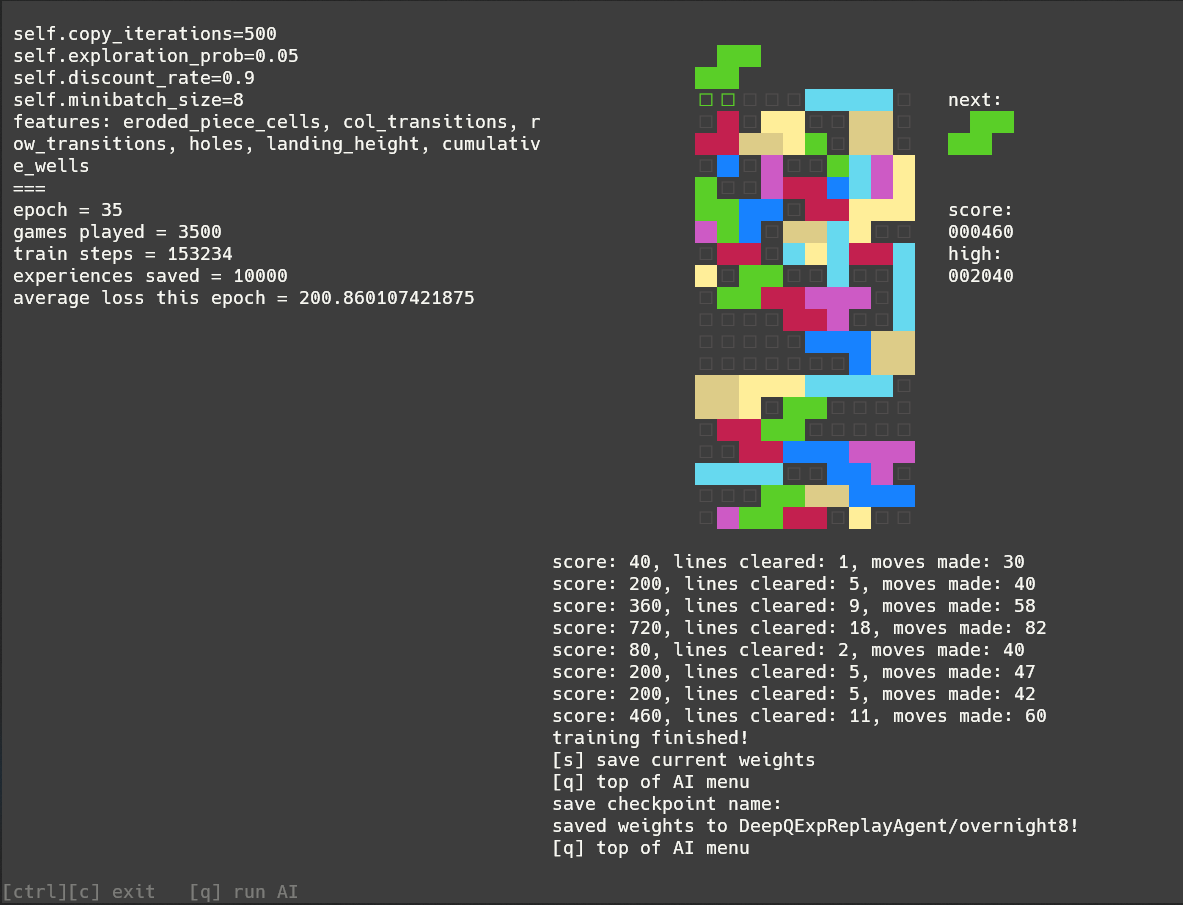
\includegraphics{sirtet_screenshot.png}
\caption{image.png}
\end{figure}

    The Sir Tet AI playground is implemented in Python with curses, so it
can run in almost any terminal with color support, without the need for
GUI functionality. It is designed for modularity and extensibility, with
plug-and-play addition of agents which must only implement a
\texttt{get\_best\_move} method, and the ability to watch agents play in
real time as they train. In addition, you can play Tetris in your
terminal.

\hypertarget{agent-features}{%
\subsection{Agent features}\label{agent-features}}

Agents are implemented as python classes (inheriting from
\texttt{BaseTetrisAgent}) and can be installed with a simple addition to
\texttt{AIRunner} in \texttt{ai\_runner.py}:

\begin{Shaded}
\begin{Highlighting}[]
\KeywordTok{class}\NormalTok{ AIRunner(Runner):}
    
\NormalTok{    installed_agents : }\StringTok{'list[tuple[BaseTetrisAgent, set]]'} \OperatorTok{=}\NormalTok{ [}
\NormalTok{        (TetrisQLearningAgent,  \{Options.TRAINABLE\}),}
\NormalTok{        (DellacherieAgent,      \{\}),}
\NormalTok{        (DeepQAgent,            \{Options.TRAINABLE, Options.MONITOR, Options.SAVABLE\}),}
\NormalTok{        (DeepQExpReplayAgent,   \{Options.TRAINABLE, Options.MONITOR, Options.SAVABLE\})}
\NormalTok{    ]}
\end{Highlighting}
\end{Shaded}

Agent initiailizers must take one positional argument which is a
\texttt{logging.Logger} object.

At minimum, an installed agent with a \texttt{get\_best\_move} method
will support watching the agent play Tetris. While watching the agent,
scores of individual games are printed out and a high score is tracked.
The method should return a legal \texttt{(orientation,\ column)} integer
pair.

Agents with \texttt{Options.TRAINABLE} set must implement a
\texttt{train(n\_iters)} method which runs \texttt{n\_iters} iterations
of a training step. For the Q-learning approaches here, this iteration
count corresponds to number of games to play, but other approaches could
interpret this parameter in any other reasonable way. The training is
done in a separate thread, while a (much slower) foreground thread
displays a live view of the agent continuously playing games with its
current training state, so the user can watch their agent learn and
improve.

Agents with \texttt{Options.SAVABLE} must implement
\texttt{save(filename)} and \texttt{load(filename)} methods to save and
load their state. For example, Keras-based agents can use
\texttt{model.save\_weights} and \texttt{model.load\_weights}. When the
user chooses to save or load weights, the checkpoint name they provide
will be prepended with a directory named after the agent's class name
before being sent to the \texttt{save} or \texttt{load} method
(e.g.~\texttt{DeepQAgent/checkpoint}).

Finally, \texttt{Options.MONITOR} indicates that an agent has a
\texttt{monitor()} method, which can be polled by the controller to
retrieve arbitrary context about the current state of the agent for
display to the user. The screenshot above shows an example of this,
where the left panel contains information about hyperparameters and
training statistics provided by the agent's \texttt{monitor()} method.

\hypertarget{recording-demonstrations}{%
\subsection{Recording demonstrations}\label{recording-demonstrations}}

The Sir Tet playground lets you record demonstrations for agents that
might require player data for pretraining steps (for example, Deep
Q-Learning from Demonstrations). After entering the demonstration
screen, you play Tetris for as long as you want, and when you choose to
save them, a text file under \texttt{demonstrations/TIMESTAMP.demo} will
be created. The format of of this text file consists of state-action
pairs separated by newlines. The state is encoded by treating each row
of the board as a 10-bit integer, concatenating the base 10
representations of the rows and appending the letter represenations of
the current tetromino and next tetromino (from the set
\texttt{zsjliot}). The action is encoded by an orientation index (for
rotation of tetromino) and a column index. Here is an example of the
demonstration syntax:

\begin{verbatim}
96/48/48/48/60/48/16/16/48/32/56/48/56/16/48/24/0/0/0/0|j|l:0,4
\end{verbatim}

Helper functions for loading demonstrations from a file into memory are
still in progress.

\hypertarget{sir-tet-architecture}{%
\subsection{Sir Tet architecture}\label{sir-tet-architecture}}

\hypertarget{game-classes}{%
\subsubsection{Game classes}\label{game-classes}}

The \texttt{TetrisGameState} consists of a \texttt{TetrisBoard}, a
current \texttt{Tetromino} and the next \texttt{Tetromino}.

A \texttt{TetrisBoard} is internally represented as a list of lists, but
can be queried by indexing it with a coordinate tuple
(\texttt{board{[}x,\ y{]}}). The return value of this indexing operation
is truthy if the cell is occupied and falsy if it is empty. Spaces
outside the board are empty.

\texttt{Tetromino}es can be indexed with an orientation index to receive
an \texttt{OrientedTetromino}, which itself can be indexed relative to
its bottom left cell with a coordinate tuple to check if that cell is
occupied by the tetromino in its current orientation. For example, a
\texttt{z} piece in orientation \texttt{0} will return \texttt{1} when
indexed at \texttt{(1,\ 0)}, \texttt{(2,\ 0)}, \texttt{(0,\ 1)} or
\texttt{(0,\ 2)}, and \texttt{0} at any other coordinate pair.

Moves are represented by pairs of integers representing orientation
index and column index.

\hypertarget{useful-methods}{%
\subsubsection{Useful methods}\label{useful-methods}}

An agent may use the following methods to aid in making its decisions:

\texttt{TetrisGameState.generate\_move\_context(orient,\ col)}: given a
move, return \texttt{gameover,\ dummy,\ yi,\ cleared}. \texttt{gameover}
is a bool which is \texttt{True} if the move resulted in a game over,
and the other return values will be \texttt{None}. \texttt{dummy} is an
instance of \texttt{TetrisBoard} with the move completed. It can be
modified arbitrarily by the agent. \texttt{yi} is the column index at
which the bottom left corner of the tetromino was placed.
\texttt{cleared} is a list of row indices that were cleared by the move.

\texttt{TetrisBoard.test\_place\_tetromino(tet\ :\ Tetromino,\ orient,\ col)}:
given a tetromino and a move, return \texttt{dummy,\ yi,\ cleared} or
raise \texttt{GameOver}. Used by
\texttt{TetrisGameState.generate\_move\_context}.

\texttt{TetrisBoard.score(cleared)}: given a list of cleared line
indices, return the score rewarded.

\texttt{TetrisGameState.get\_moves()}: generator that yields all valid
\texttt{(orient,\ col)} pairs. Note that moves that can cause a
\texttt{GameOver} are still considered valid.

Other methods of a \texttt{TetrisGameState} or its \texttt{TetrisBoard}
should not be used by agents as they may mutate the controller's state.

\hypertarget{writing-features}{%
\subsubsection{Writing features}\label{writing-features}}

Feature extractors of a state or state action pair may use the methods
discussed above. Many features are implemented in \texttt{features.py}
and \texttt{features2.py} (the latter of which has cleaner code). Here
is an example feature:

\begin{Shaded}
\begin{Highlighting}[]
\KeywordTok{def}\NormalTok{ holes(state : TetrisGameState, orient, col):}
    \CommentTok{'''}
\CommentTok{    count number of holes in board resulting from action (normalized to [0, 1])}
\CommentTok{    '''}
    
    \CommentTok{#this preamble is standard for move-agnostic features}
\NormalTok{    gameover, board, _, _ }\OperatorTok{=}\NormalTok{ state.generate_move_context(orient, col)}
    \ControlFlowTok{if}\NormalTok{ gameover:}
        \ControlFlowTok{return} \DecValTok{0}

\NormalTok{    h }\OperatorTok{=} \DecValTok{0}
    \ControlFlowTok{for}\NormalTok{ x, y }\KeywordTok{in}\NormalTok{ board.coords():}
        \ControlFlowTok{if} \KeywordTok{not}\NormalTok{ board[x, y]:}
            \ControlFlowTok{for}\NormalTok{ ty }\KeywordTok{in} \BuiltInTok{range}\NormalTok{(y }\OperatorTok{+} \DecValTok{1}\NormalTok{, HEIGHT):}
                \ControlFlowTok{if}\NormalTok{ board[x, ty]:}
\NormalTok{                    h }\OperatorTok{+=} \DecValTok{1}
                    \ControlFlowTok{break}
    \ControlFlowTok{return}\NormalTok{ h}\OperatorTok{/}\DecValTok{200}
\end{Highlighting}
\end{Shaded}

\hypertarget{runners-and-userinterface}{%
\subsubsection{\texorpdfstring{\texttt{Runner}s and
\texttt{UserInterface}}{Runners and UserInterface}}\label{runners-and-userinterface}}

The Sir Tet playground consists of three \texttt{Runner}s found in
\texttt{*\_runner.py} which control the \texttt{UserInterface} object
responsible for rendering the screen to the user. The latter has methods
that make extending the platform more tractable, allowing easy
displaying of text, prompting for strings, and manipulating the visible
Tetris game.

    \hypertarget{tetris-agents}{%
\section{Tetris Agents}\label{tetris-agents}}

After the poor performance of the linear Q-learning agent from a few
months ago, where there was difficulty in selecting a good feature set
and tuning hyperparameters, I wanted to try the approach of taking the
proven feature set of Dellacherie (that still outperforms many more
complex approaches) and seeing if a non-linear, neural optimization
function would achieve better results than the linear function.

\hypertarget{dellacheries-agent}{%
\subsection{Dellacherie's agent}\label{dellacheries-agent}}

Dellacherie's agent, as described earlier, simply picks the move that
optimizes the following formula:

    \(\text{eroded piece cells} - \text{col transitions} - \text{row transitions} - \text{landing height} - \text{cumulative wells} - 4\cdot\text{holes}\)

    Some of these features are move-agnostic (i.e.~features of the resulting
board state only) while others are dependent on the move.

\texttt{eroded\_piece\_cells}: number of lines cleared by move * number
of bricks of placed tetromino cleared (e.g.~if four lines are cleared by
an \texttt{i}, this equals 16)

\texttt{col\_transitions}: number of vertical pairs of cells which
contain both an empty cell and a block, i.e.~number of vertical
transitions from block to gap

\texttt{row\_transitions}: similar to \texttt{col\_transitions}

\texttt{landing\_height}: height at which placed piece lands
(=\texttt{yi} from \texttt{generate\_move\_context})

\texttt{cumulative\_wells}:
\(\sum_{w\in wells} (1 + 2 + ... + depth(w))\) where a well is defined
as a vertical sequence of empty cells with blocks on the left and right.

\texttt{holes}: number of holes where a hole is defined as an empty cell
with at least one block above it in the same column.

The implementation of this agent was simple once the features were
implemented:

\begin{Shaded}
\begin{Highlighting}[]
\KeywordTok{class}\NormalTok{ DellacherieAgent(BaseTetrisAgent):}

\NormalTok{    agent_name }\OperatorTok{=} \StringTok{'Dellacherie}\CharTok{\textbackslash{}'}\StringTok{s legendary hand coded agent'}

\NormalTok{    weights : }\StringTok{'dict[Callable[[TetrisGameState, int, int], float], float]'} \OperatorTok{=}\NormalTok{ \{}
\NormalTok{        eroded_piece_cells: }\FloatTok{1.0}\NormalTok{,}
\NormalTok{        col_transitions: }\FloatTok{-1.0}\NormalTok{,}
\NormalTok{        row_transitions: }\FloatTok{-1.0}\NormalTok{,}
\NormalTok{        landing_height: }\FloatTok{-1.0}\NormalTok{,}
\NormalTok{        cumulative_wells: }\FloatTok{-1.0}\NormalTok{,}
\NormalTok{        holes: }\FloatTok{-4.0}
\NormalTok{    \}}

    \KeywordTok{def} \FunctionTok{__init__}\NormalTok{(}\VariableTok{self}\NormalTok{, logger):}
        \VariableTok{self}\NormalTok{.logger }\OperatorTok{=}\NormalTok{ logger}

    \KeywordTok{def}\NormalTok{ get_best_move(}\VariableTok{self}\NormalTok{, state: TetrisGameState) }\OperatorTok{->} \StringTok{'tuple[int, int]'}\NormalTok{:}
\NormalTok{        moves }\OperatorTok{=} \BuiltInTok{list}\NormalTok{(state.get_moves())}
\NormalTok{        move_scores }\OperatorTok{=}\NormalTok{ \{(orient, col): }\BuiltInTok{sum}\NormalTok{(w}\OperatorTok{*}\NormalTok{f(state, orient, col) }\ControlFlowTok{for}\NormalTok{ f, w }\KeywordTok{in} \VariableTok{self}\NormalTok{.weights.items())}
            \ControlFlowTok{for}\NormalTok{ orient, col }\KeywordTok{in}\NormalTok{ moves\}}
        \ControlFlowTok{return} \BuiltInTok{max}\NormalTok{(moves, key}\OperatorTok{=}\KeywordTok{lambda}\NormalTok{ m: move_scores[m])}
\end{Highlighting}
\end{Shaded}

\hypertarget{deep-q-learning-naive}{%
\subsection{Deep Q-Learning (naive)}\label{deep-q-learning-naive}}

This first approach to Deep Q-Learning uses a Q-value estimator network
which takes the extracted features of a state-action pair as inputs and
outputs a single Q value. The feature set was kept the same as
Dellacherie's. The model consists of two fully connected hidden layers
with 16 hidden units. There is also a target network to which the
weights of the estimator are copied every 100 training steps. On each
training step, the estimator chooses an action using the
\(\epsilon\)-greedy approach, and then calculates the loss

\[l = (r_{s,a,s'} + max_{a'}\hat{Q}(s', a') - Q(s, a))^2\]

where \(Q\) is the estimator model, \(\hat{Q}\) is the target model, and
\(r\) is the reward obtained in the transition resulting from the chosen
action. This loss is used to update the weights of the estimator network
using the \texttt{keras.optimizers.Adam} optimizer.

\hypertarget{deep-q-learning-with-experience-replay}{%
\subsection{Deep Q-learning with Experience
Replay}\label{deep-q-learning-with-experience-replay}}

After some reading, I realized that one common approach in Deep
Q-learning is to randomly sample from past experiences to mitigate some
of the correlation found in a standard sequential learning approach.
This agent stores a buffer of observed state transitions (storing the
input to the network instead of the actual state action pair), and at
each training step samples a minibatch of experiences from the replay
buffer, calculates the loss of the entire batch with respect to the
current states of the estimator and target model, and performs
optimization with these losses.

\hypertarget{results}{%
\subsection{Results}\label{results}}

The Deep Q learning agents were trained for 8 hours each on
approximately 3500 games. The experience replay model was trained with
three different sets of hyperparameters, the best one being
\texttt{copy\_iterations=250} and \texttt{minibatch\_size=64}.

\begin{longtable}[]{@{}lll@{}}
\toprule
Agent & Average score (last 12 games) & High Score\tabularnewline
\midrule
\endhead
Dellacherie & 41560 & 194060\tabularnewline
Deep Q Learning & 365 & 2940\tabularnewline
DQL with ER & 423 & 3180\tabularnewline
\bottomrule
\end{longtable}

    \hypertarget{discussion-and-future-work}{%
\section{Discussion and future work}\label{discussion-and-future-work}}

The results are surprisingly poor considering the feature set used was
the same as Dellacherie's agent. I expected the networks to be able to
at least match Dellacherie's performance by approximating a linear
function of the features.

One of the reasons for this poor performance might be insufficient
training time. Even after eight hours of training, the average losses
were in the hundreds. This might indicate that longer training times or
larger batches of experiences should be used, or some of the learning
rates need to be tweaked to obtain faster convergence. Alternatively,
maybe the target network is still moving too fast for the estimator to
converge to it. I was unable to test all of these factors due to time
constraints.

A possible improvement might be made by implementing Deep Q-Learning
from demonstrations. Kick-starting the learning process with a set of
user-recorded demonstrations might help the model by starting it off
with a reasonable understanding of the strategy and allowing it to catch
up to Dellacherie in performance. Unfortunately, because of time
constraints, I was unable to implement the usage of recorded
demonstrations in this project's timeframe.

Of course, it's possible that the feature sets used in these models are
the culprit--maybe Dellacherie's features are not suited to a complex
non-linear optimizer. Maybe reducing the complexity of the network or
trying different feature sets would have some positive impact on
performance.

Lastly, it's possible that Q-learning based approaches are simply
infeasible for Tetris. This might be a result of the long sequences of
actions without any rewards making it difficult to quickly get accurate
Q-value estimates. Perhaps some form of reward shaping might combat
this, but perhaps the reason the literature is light on Q-learning for
Tetris is that it simply isn't a good solution for the problem.

Hopefully whoever next tackles this problem will find the Sir Tet
Playground and the agents I implemented useful.

    \hypertarget{references}{%
\section{References}\label{references}}

{[}1{]} Fahey, C. P. (2003). Tetris AI, Computer plays Tetris.
http://colinfahey.com/tetris/tetris\_en.html

{[}2{]} Bohm, N., Kokai, G., and Mandl, S. (2005). An Evolutionary
Approach to Tetris. \emph{The Sixth Metaheuristics International
Conference (MIC2005).}

{[}3{]} Da Silva, R. S., and Parpinelli, R. S. (2017). Playing the
Original Game Boy Tetris Using a Real Coded Genetic Algorithm.
\emph{2017 Brazilian Conference on Intelligent Systems.}

{[}4{]} Lagoudakis, M. G., Parr, R., and Littman, M. L. (2002).
Least-squares methods in reinforcement learning for control.
\emph{Hellenic Conference on Artificial Intelligence.}

{[}5{]} Chen, X., Wang, H., Wang, W., Shi, Y., and Gao, Y. (2009). Apply
ant colony optimization to tetris. \emph{Proceedings of the 11th Annual
conference on Genetic and evolutionary computation.}

{[}6{]} Langenhoven, L., Van Heerden, W. S., and Engelbrecht, A. P.
(2010). Swarm tetris: Applying particle swarm optimization to tetris.
\emph{Evolutionary Computation (CEC), 2010 IEEE Congress on.}

{[}7{]} Thiery, C., Scherrer, B. (2009). Building Controllers for
Tetris. \emph{International Computer Games Association Journal}

{[}8{]} Carr, D. (2005). Applying reinforcement learning to Tetris.
\emph{Rhodes University}


    % Add a bibliography block to the postdoc
    
    
    
\end{document}
